\documentclass{article}
\usepackage{listings}
\usepackage{ctex}
\usepackage{graphicx}
\usepackage[a4paper, body={18cm,22cm}]{geometry}
\usepackage{amsmath,amssymb,amstext,wasysym,enumerate,graphicx,caption,subfigure}
\usepackage{float,abstract,booktabs,indentfirst,amsmath}
\usepackage{array}
\usepackage{booktabs} %调整表格线与上下内容的间隔
\usepackage{multirow}
\usepackage{url}
\usepackage{diagbox}
\renewcommand\arraystretch{1.4}
\usepackage{indentfirst}
\setlength{\parindent}{2em}
\usepackage{listings}
\usepackage{xcolor}
\lstset{
	numbers=left, 
	numberstyle= \tiny, 
	keywordstyle= \color{ blue!70},
	commentstyle= \color{red!50!green!50!blue!50}, 
	frame=shadowbox, % 阴影效果
	rulesepcolor= \color{ red!20!green!20!blue!20} ,
	escapeinside=``, % 英文分号中可写入中文
	xleftmargin=2em,xrightmargin=2em, aboveskip=1em,
	basicstyle=\footnotesize,
	framexleftmargin=2em
} 


\geometry{left=2.8cm,right=2.2cm,top=2.5cm,bottom=2.5cm}
%\geometry{left=3.18cm,right=3.18cm,top=2.54cm,bottom=2.54cm}

\graphicspath{{figures/}}

\title{\heiti 数字电路实验报告 }

\begin{document}
	\vspace*{1cm}
	
	\begin{figure}[h]
		\centering
		
\includegraphics[scale=1.0]{xh.jpg}
	\end{figure}

	\vspace*{0.5cm}
	
	\begin{center}
		\Huge{\textbf{数字电路实验报告}}
	\end{center}
	
	\vspace{5cm}
	
	\begin{table}[h]
		\centering
		\begin{Large}
			\begin{tabular}{p{3cm} p{7cm}<{\centering}}
				实验题目: &  Verilog 硬件描述语言     \\ \cline{2-2}
				学生姓名:      & 孔浩宇   \\ \cline{2-2}
				学生学号: & PB20000113 \\ \cline{2-2}
				完成日期:       & 2022/11/2 \\ \cline{2-2}
			\end{tabular}
		\end{Large}		
	\end{table}
	\newpage
    \section{实验题目}
        \subsection*{\qquad Verilog 硬件描述语言}

    \section{实验目的}
        \subsection*{\qquad (1)掌握 Verilog HDL 常用语法}
        \subsection*{\qquad (2)能够熟练阅读并理解 Verilog 代码}
        \subsection*{\qquad (3)能够设计较复杂的数字功能电路}
        \subsection*{\qquad (4)能够将 Verilog 代码与实际硬件相对应}
        
    \section{实验环境}
        \subsection*{\qquad (1) vlab.ustc.edu.cn}
        \subsection*{\qquad (2) verilog.ustc.edu.cn}
    
    \section{实验练习}
    \subsection*{题目1} if\ldots else只能用在always语句内部.
	\begin{figure}[htbp]
		\centering
		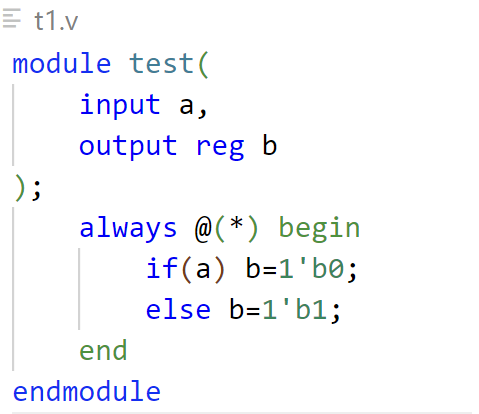
\includegraphics[scale=1]{t1.png}
		\caption*{题目1}
	\end{figure}
	\clearpage
    \subsection*{题目2} 如图
	\begin{figure}[htbp]
		\centering
		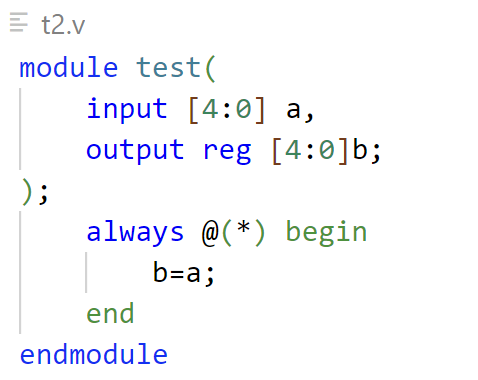
\includegraphics[scale=1]{t2.png}
		\caption*{题目2}
	\end{figure}

    \subsection*{题目3} 如图
	\begin{figure}[htbp]
		\centering
		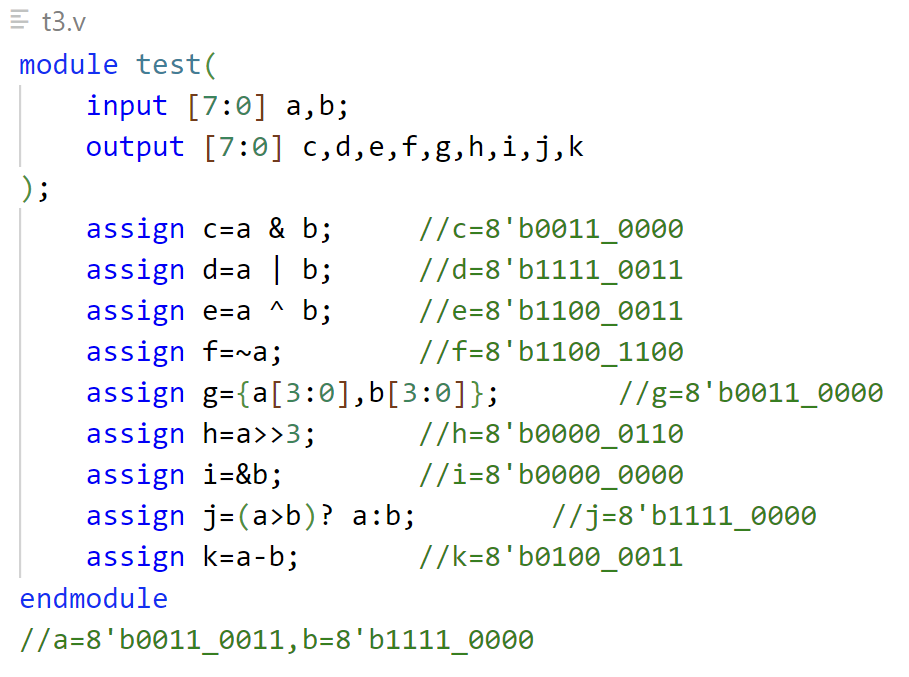
\includegraphics[scale=0.8]{t3.png}
		\caption*{题目3}
	\end{figure}
	\clearpage
    \subsection*{题目4}	assign不能给reg赋值;模块实例化格式错误
	\begin{figure}[htbp]
		\centering
		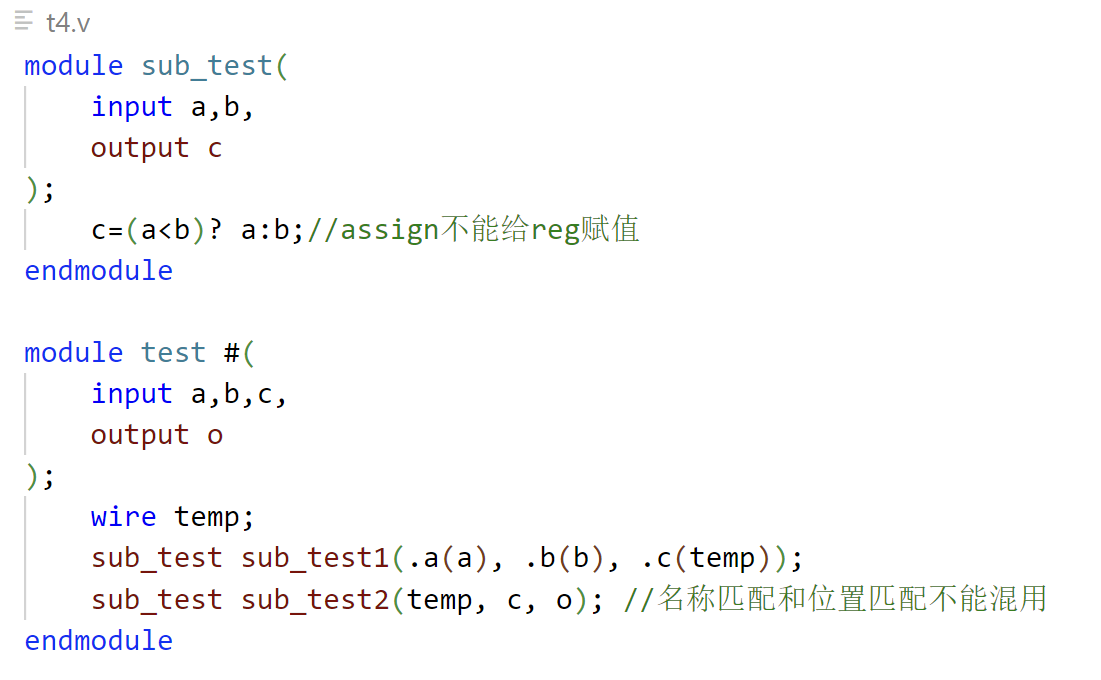
\includegraphics[scale=0.8]{t4.png}
		\caption*{题目4}
	\end{figure}

    \subsection*{题目5} 端口定义不准确,模块实例化不能存在于always语句中
	\begin{figure}[htbp]
		\centering
		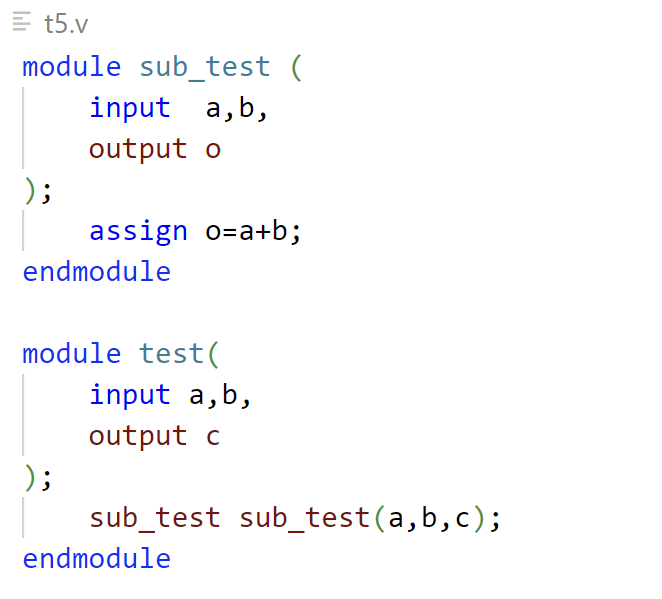
\includegraphics[scale=0.6]{t5.png}
		\caption*{题目5}
	\end{figure}

	\clearpage
    \section{总结与思考}
	\begin{enumerate}
		\item [1.]基本掌握了verilog语法,能够自主理解并编写verilog代码
		\item [2.]本次实验难度适中
		\item [3.]本次实验任务量适中
		\item [4.]可以多给点硬件的实例
	\end{enumerate}
\end{document}